\documentclass[11pt,a4paper]{article}

\usepackage[T1]{fontenc}
\usepackage[utf8]{inputenc}
\usepackage[english]{babel}
\usepackage{lmodern}
\usepackage{amsmath,amssymb,amsfonts}
\usepackage{booktabs}
\usepackage{geometry}
\usepackage{graphicx}
\usepackage{microtype}
\usepackage{enumitem}
\usepackage[numbers,sort&compress]{natbib}
\usepackage{caption}
\usepackage{hyperref}

\geometry{margin=1in}
\hypersetup{
  hidelinks,
  pdftitle={Transport Graph Lab Demo},
  pdfauthor={Pedro Henrique}
}
\setlist[itemize]{leftmargin=1.4em}
\setlist[enumerate]{leftmargin=1.6em}
\captionsetup{font=small,labelfont=bf}

\title{\textbf{Transport Graph Lab Demo}\\
\large Coherent and Dissipative Transport in Simple Open Quantum Networks}
\author{Pedro Henrique}
\date{April 2026}

\begin{document}

\maketitle

\begin{abstract}
This short report documents the numerical experiments currently implemented in
the transport-graph laboratory. The goal is to compare simple graph topologies
under the same open-system model, to explain what the sink represents, and to
show how the main observable (sink efficiency) changes when the dephasing rate
is varied. The baseline comparison includes a complete graph, a ring, and a
chain, with population dynamics and coherence used as secondary diagnostics.
\end{abstract}

\section{What these experiments are}

The present numerical experiments are not laboratory measurements. They are
controlled open-system simulations designed to answer a clean physics question:
how graph topology changes transport toward a target channel when coherent
hopping competes with decoherence.

Each simulated experiment follows the same logic:
\begin{enumerate}
  \item choose a graph topology;
  \item prepare one initial excitation on a selected site;
  \item evolve the state with coherent hopping plus dissipative channels;
  \item measure how much population reaches the sink;
  \item compare the result across dephasing rates and topologies.
\end{enumerate}

\section{Physical model and references}

The network is described in the single-excitation sector by the tight-binding
Hamiltonian
\begin{equation}
H = \sum_{i=1}^{N}\epsilon_i |i\rangle\langle i|
  + \sum_{i\neq j} J_{ij}|i\rangle\langle j|.
\end{equation}

Open-system evolution is modeled with the Lindblad master equation
\begin{equation}
\frac{d\rho}{dt}
= -i[H,\rho]
+ \sum_k \left(
L_k \rho L_k^\dagger - \frac{1}{2}\{L_k^\dagger L_k,\rho\}
\right),
\end{equation}
which is the standard minimal framework for a first study of coherent and
dissipative transport in small open systems
\citep{breuer_petruccione_2007,rivas_huelga_2012}.

The transport-specific motivation comes from the literature on
dephasing-assisted or environment-assisted transport in quantum networks
\citep{mohseni_2008,plenio_huelga_2008,rebentrost_2009,caruso_2009,marais_2013,coates_2021,coates_2023}.
The optional long-term bridge to experiment is motivated by programmable quantum
platforms such as superconducting circuits
\citep{potocnik_2018,zhang_2024_transport,naeij_2025}.

\section{What the sink means}

The sink is an absorbing target state that represents successful transport. It
is not an additional graph node. Instead, it is the bookkeeping channel that
receives population from the chosen trap site. The final sink population is
therefore the transport-success metric,
\begin{equation}
\eta(T) = \rho_{ss}(T).
\end{equation}

This construction is useful because it separates:
\begin{itemize}
  \item coherent motion inside the graph;
  \item successful capture into the target channel;
  \item unwanted dissipation into a distinct loss channel.
\end{itemize}

\section{Main and secondary observables}

The main observable is the sink efficiency:
\begin{equation}
\eta(T)=\rho_{ss}(T).
\end{equation}

The secondary observables are:
\begin{equation}
P_i(t)=\rho_{ii}(t),
\end{equation}
which track population flow across the graph, and
\begin{equation}
C_{\ell_1}(\rho)=\sum_{i\neq j}|\rho_{ij}|,
\end{equation}
which provides a direct coherence diagnostic in the site basis.

\section{Baseline topologies}

The current baseline uses three families:
\begin{itemize}
  \item a complete graph, which is useful for exposing interference-assisted and
  interference-blocked pathways;
  \item a ring, which allows coherent circulation and sensitivity to disorder;
  \item a chain, which gives the simplest directional transport geometry.
\end{itemize}

\begin{figure}[t]
  \centering
  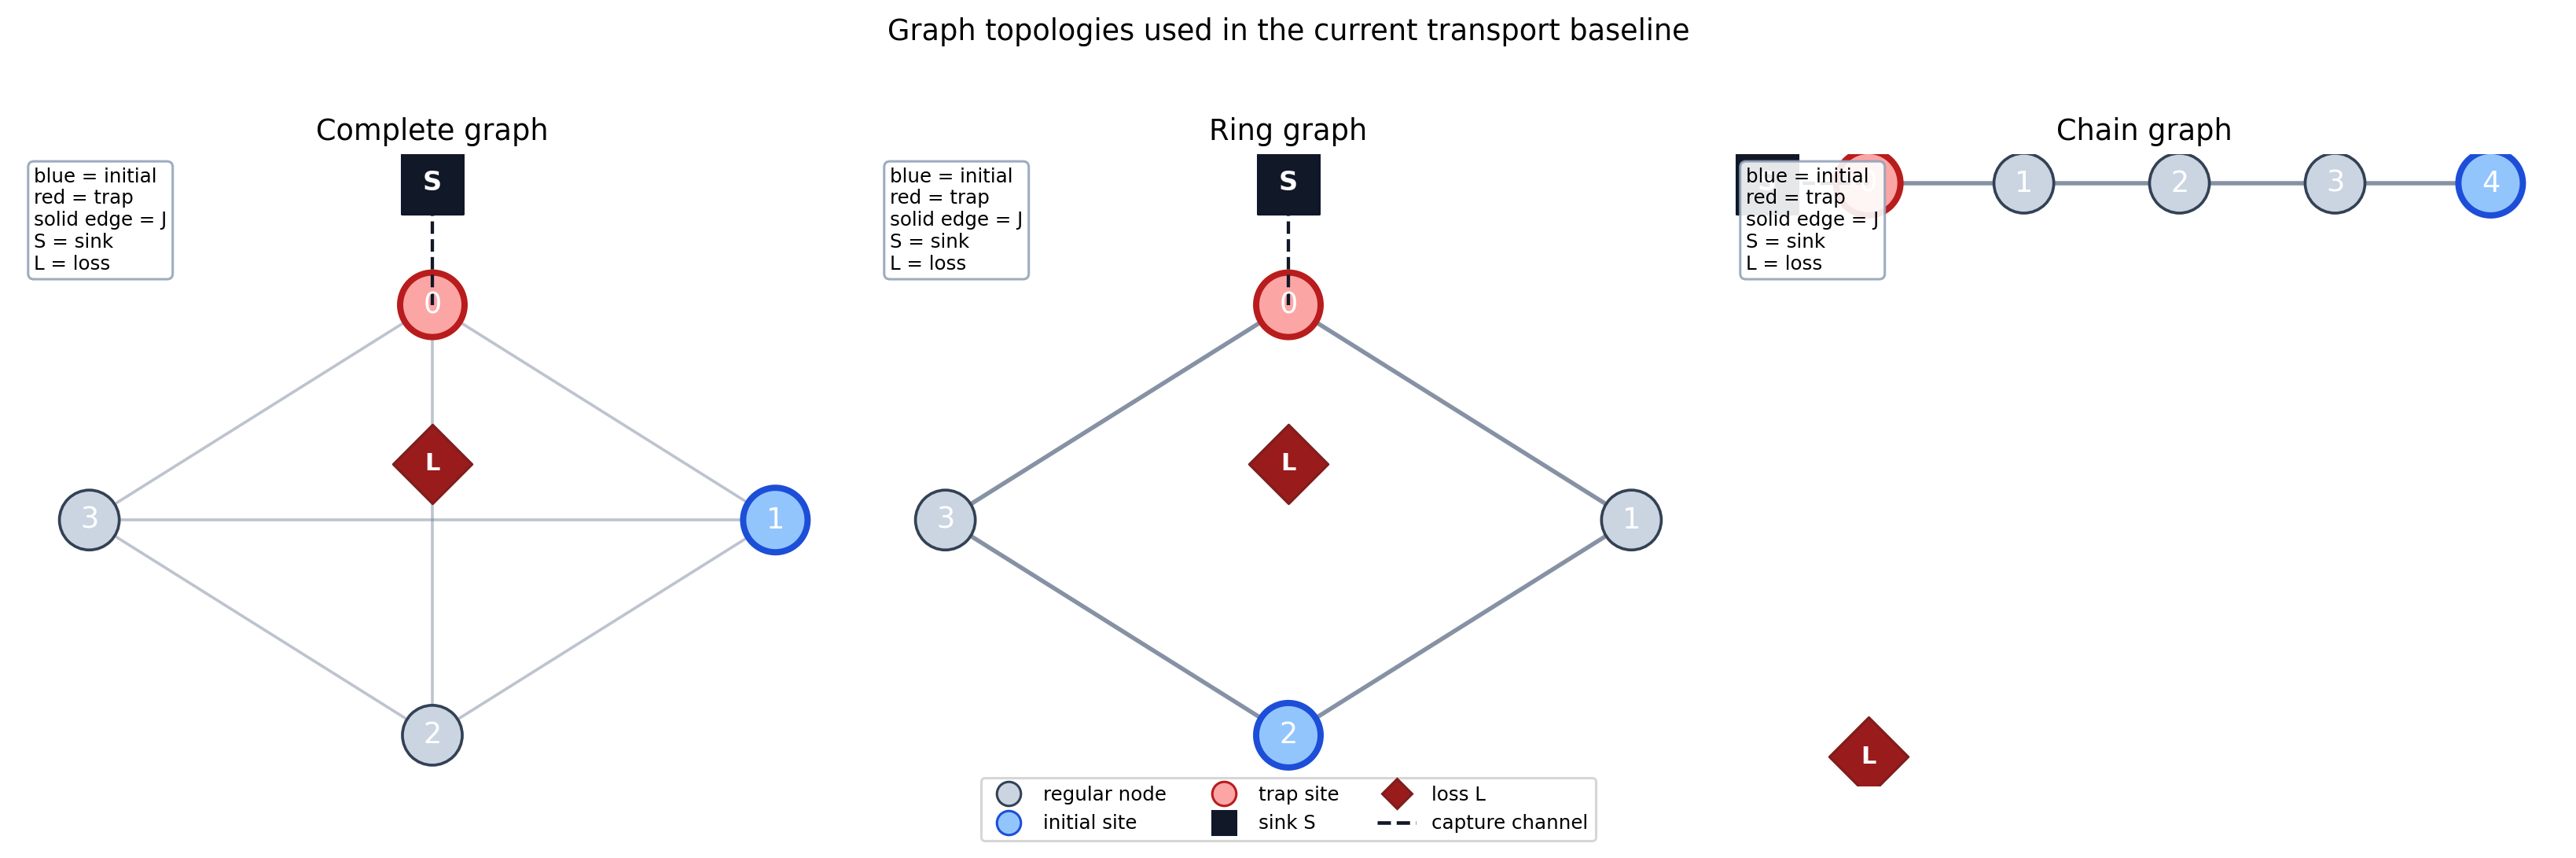
\includegraphics[width=0.96\textwidth]{../../outputs/transport_networks/graph_lab/latest/figures/graph_topology_overview.png}
  \caption{Topology overview of the graphs used in the current baseline. The
  colored nodes indicate the initial site and the trap site, while the square
  node $S$ represents the sink channel used to measure successful transport.}
\end{figure}

\section{Current simulation results}

The following table is generated automatically from the latest run of the graph
lab baseline.

\begin{table}[t]
\centering
\caption{Automatically generated summary of the current baseline graph comparison.}
\begin{tabular}{lcccc}
\toprule
Scenario & Best regime & $\eta_{\mathrm{coh}}$ & $\eta_{\mathrm{best}}$ & $\gamma_{\phi}^{\mathrm{best}}$ \\
\midrule
Complete graph & intermediate & 0.300 & 0.798 & 3.200 \\
Ring graph & coherent & 0.795 & 0.795 & 0.000 \\
Chain graph & coherent & 0.812 & 0.812 & 0.000 \\
\bottomrule
\end{tabular}
\end{table}


\begin{figure}[t]
  \centering
  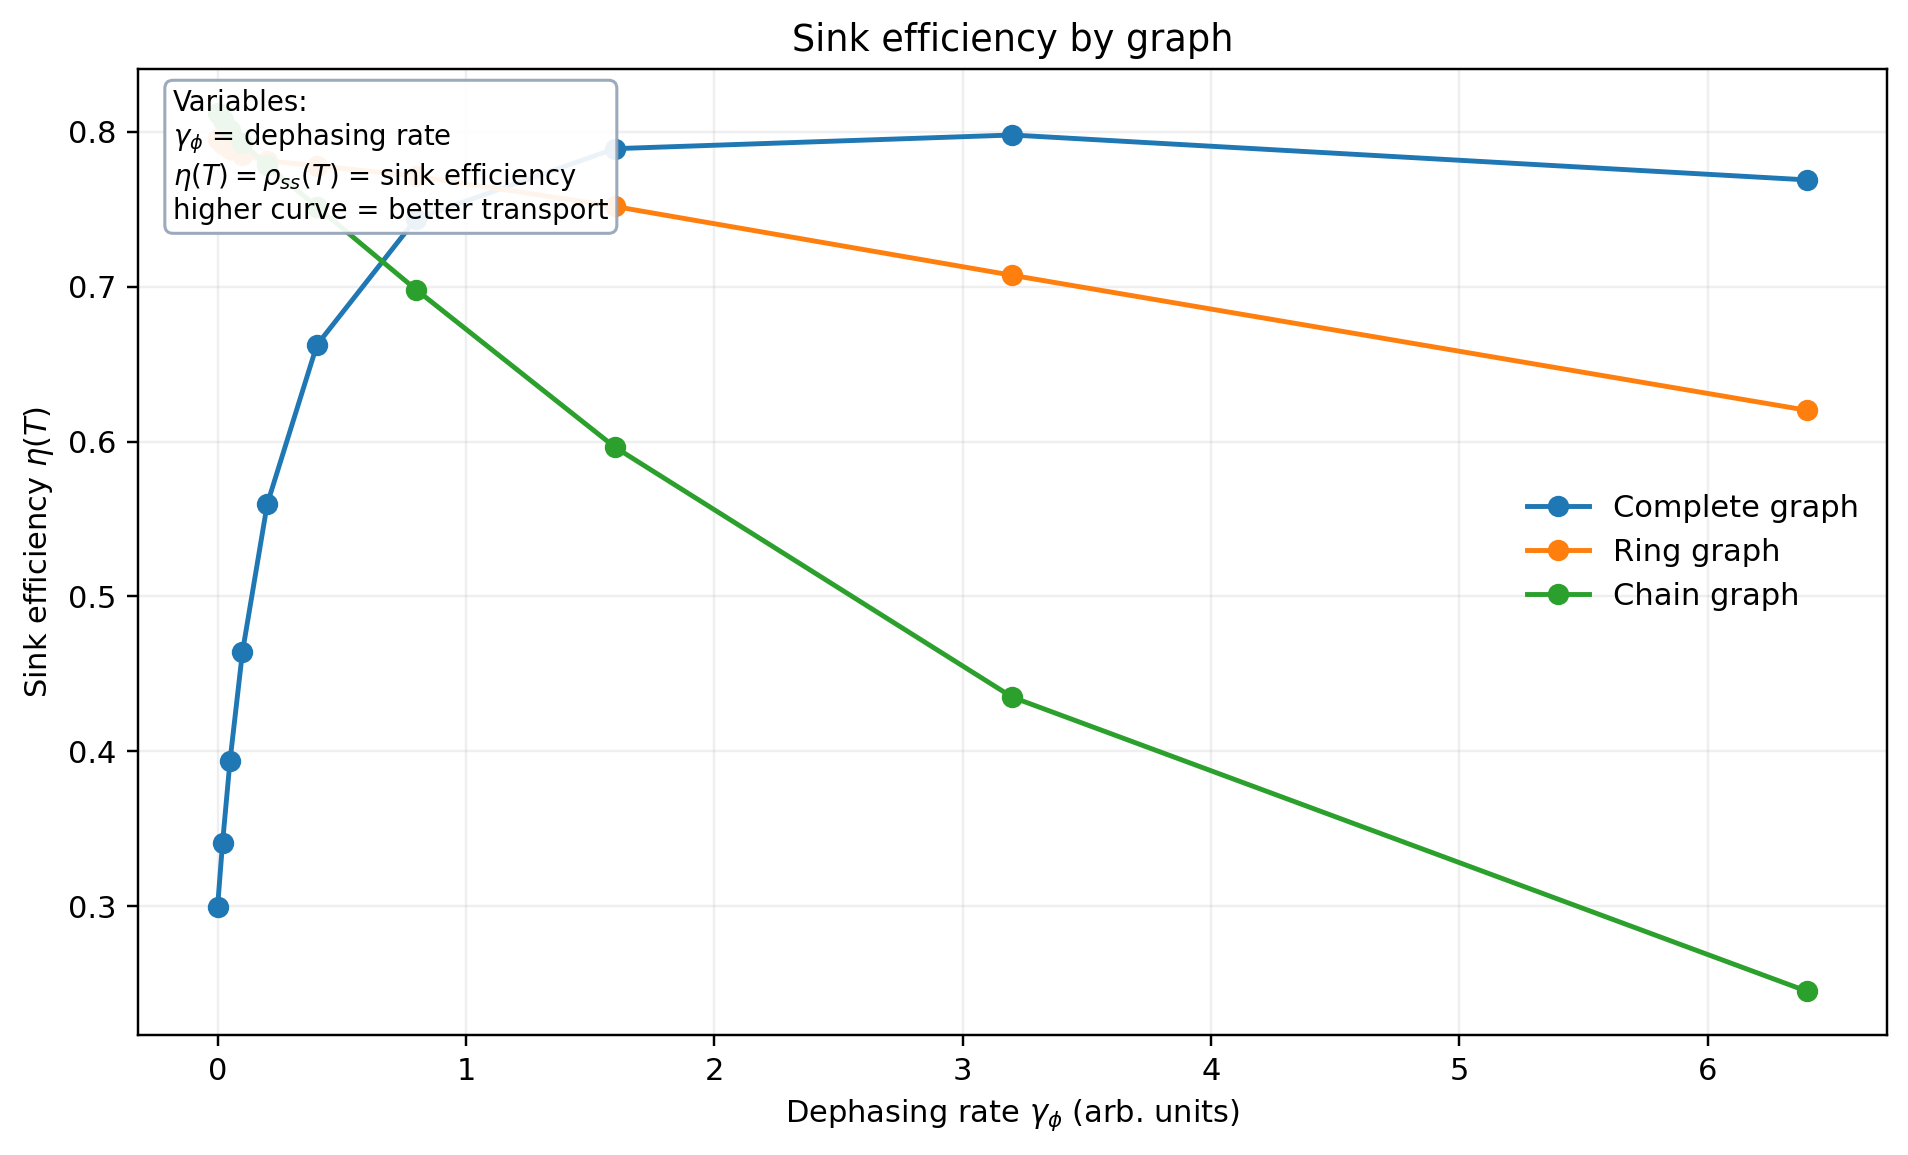
\includegraphics[width=0.92\textwidth]{../../outputs/transport_networks/graph_lab/latest/figures/sink_efficiency_by_graph.png}
  \caption{Main result: sink efficiency as a function of the dephasing rate for
  the baseline graph family comparison.}
\end{figure}

\begin{figure}[t]
  \centering
  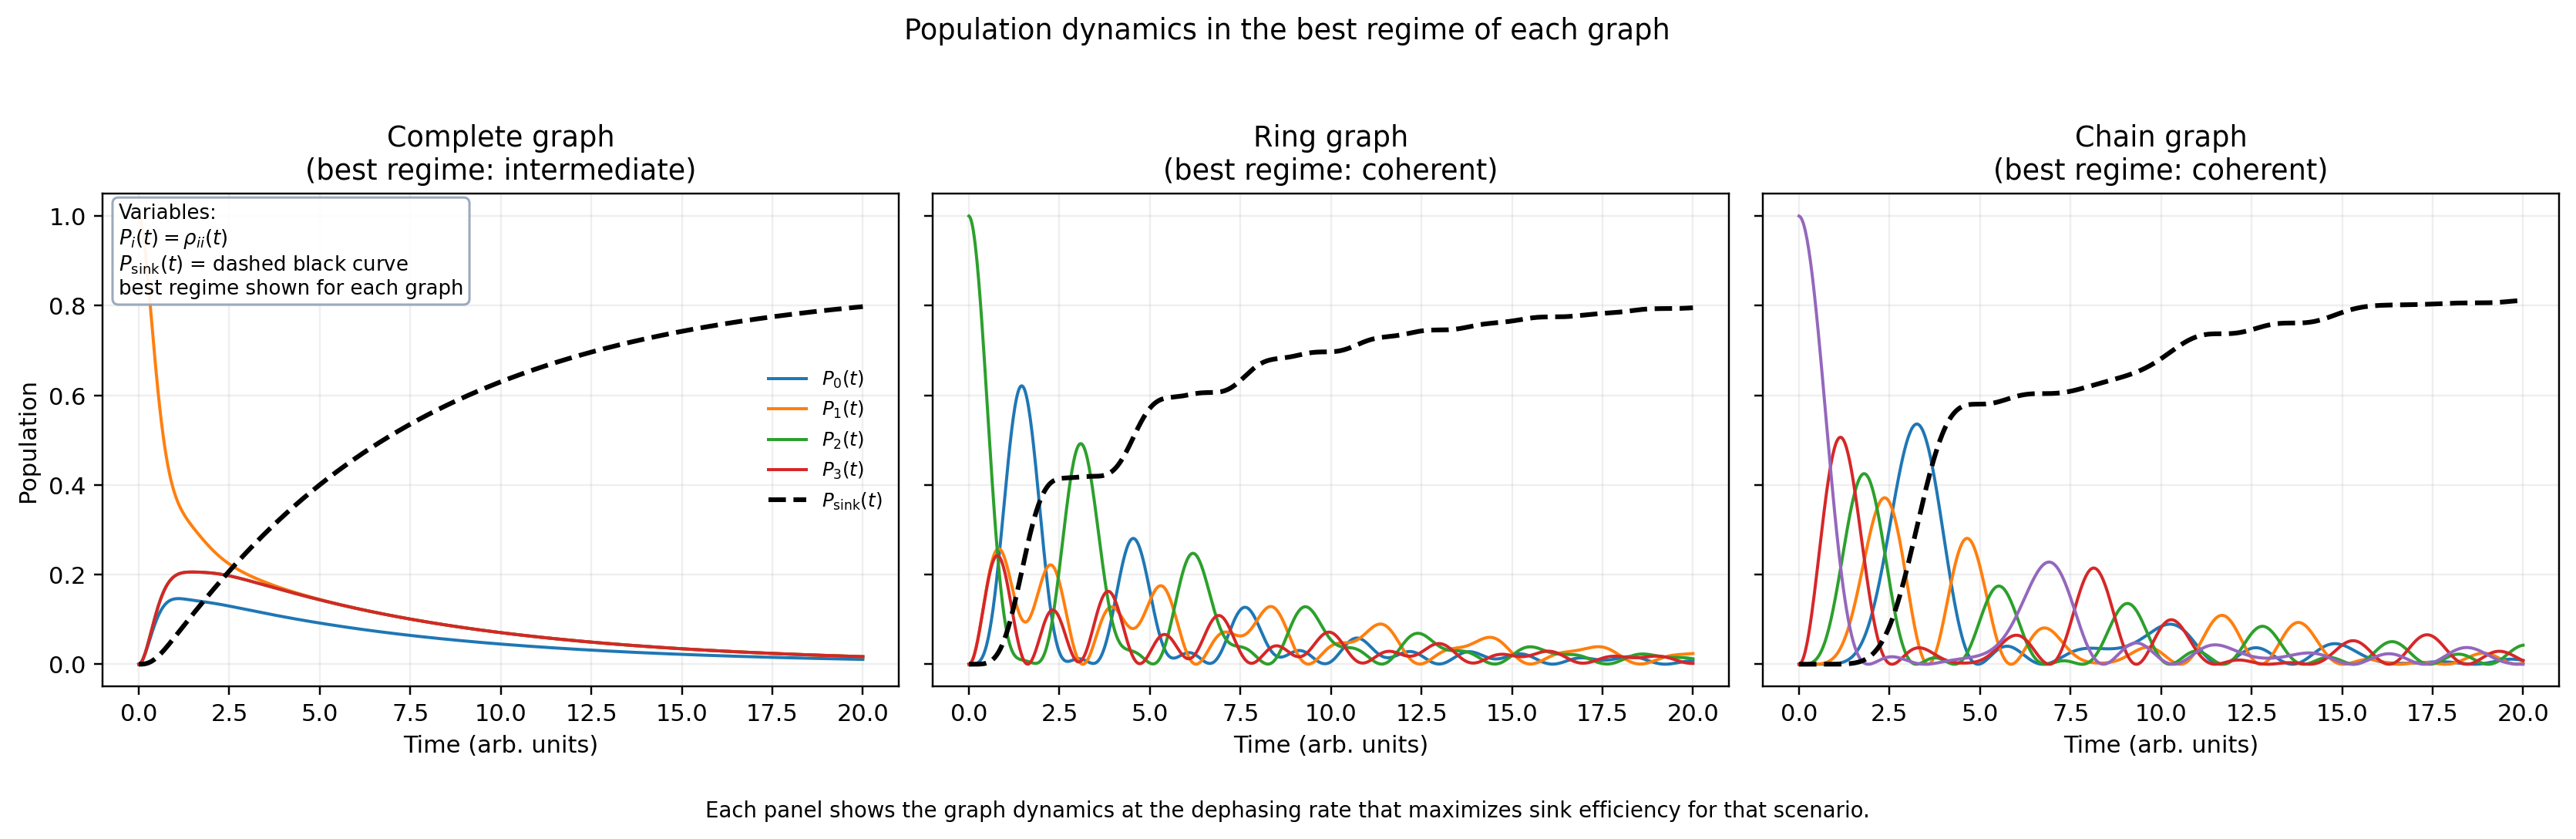
\includegraphics[width=0.95\textwidth]{../../outputs/transport_networks/graph_lab/latest/figures/population_dynamics_by_graph.png}
  \caption{Population dynamics in the best regime identified for each graph.}
\end{figure}

\begin{figure}[t]
  \centering
  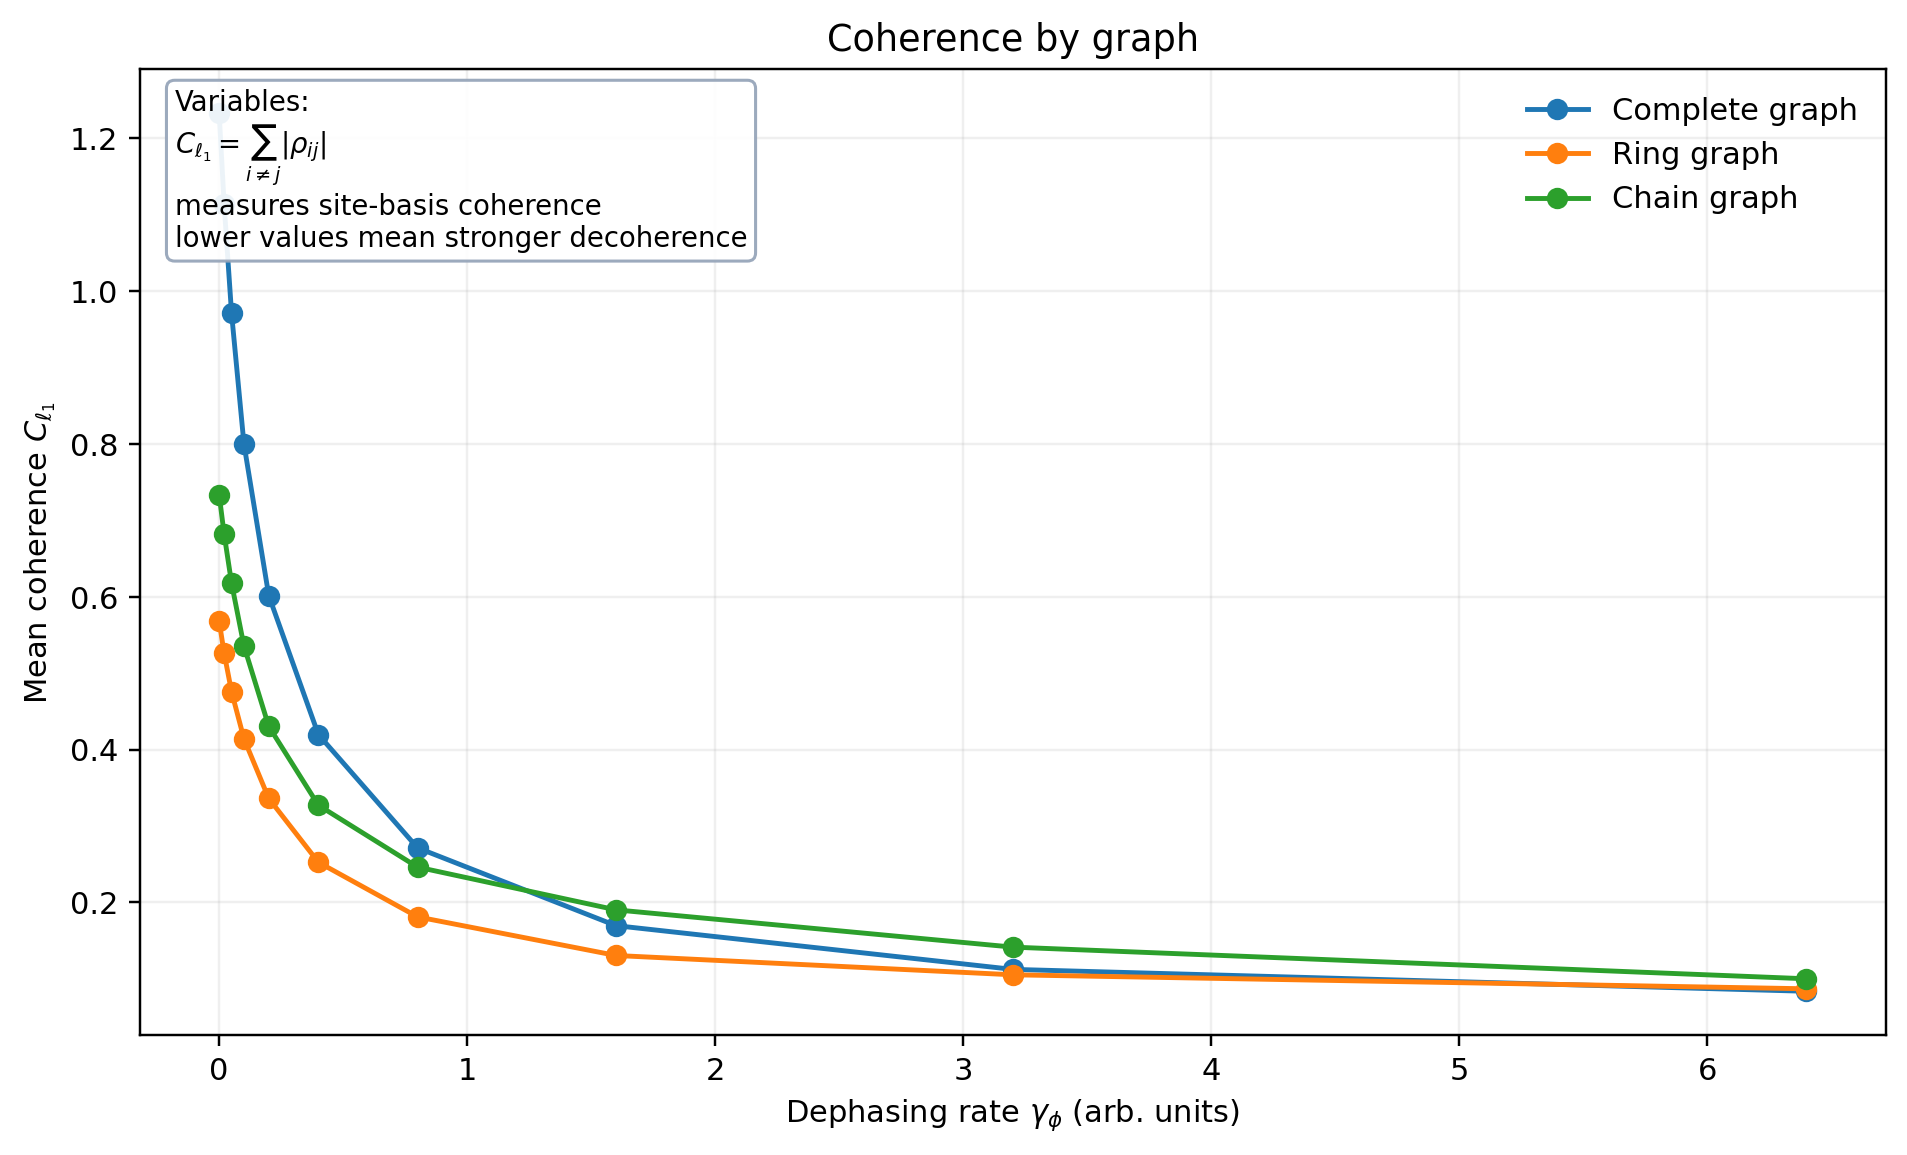
\includegraphics[width=0.92\textwidth]{../../outputs/transport_networks/graph_lab/latest/figures/coherence_by_graph.png}
  \caption{Coherence diagnostic as a function of the dephasing rate for the same
  graph family comparison.}
\end{figure}

\section{How to change the simulations}

The editable configuration file is:
\begin{quote}
\texttt{configs/transport\_graph\_lab\_config.json}
\end{quote}

The main parameters you can change are:
\begin{itemize}
  \item \texttt{seed};
  \item \texttt{n\_sites};
  \item \texttt{topology};
  \item \texttt{initial\_site};
  \item \texttt{trap\_site};
  \item \texttt{coupling\_hz};
  \item \texttt{sink\_rate\_hz};
  \item \texttt{loss\_rate\_hz};
  \item \texttt{disorder\_strength\_hz};
  \item \texttt{dephasing\_rates\_hz}.
\end{itemize}

After editing the configuration, the simulation is regenerated by running:
\begin{quote}
\texttt{python scripts\textbackslash run\_transport\_graph\_lab.py}
\end{quote}

The lab also generates one GIF animation per scenario, showing how the node
populations, sink occupation, and loss evolve in the best regime identified for
that graph.

\section{Interpretation of the current baseline}

The present baseline already shows three qualitatively different behaviors.
For the complete graph, the best regime is intermediate, which means that
moderate dephasing improves sink efficiency relative to the coherent limit.
For the ring and the chain, the best performance remains at the coherent limit,
while strong dephasing suppresses transport. This is already enough to justify
the central research direction of the project: topology and decoherence cannot
be discussed separately.

\bibliographystyle{unsrtnat}
\bibliography{references}

\end{document}
